\section{Experimental Results}
\label{sec:eval}

We conducted a series of experiments on
4 main datasets in Table \ref{tab:datasets}. BMS-POS and BMS-WebView are
introduced in \cite{Zheng:2001:RWP:502512.502572} and are commonly used for
data mining. Retail is the retail market basket data \cite{brijs99:retailData}. Syn is the synthetic data in which each item is generated with
equal probability and the max record length is 50.
%
Figure \ref{fig:datasets} shows the record length distribution of the datasets.
All the datasets exhibit a trend where the number of records decreases almost exponentially
with the record length.
%
We randomly designate 40\% of the item types in each dataset as
sensitive items and the rest as non-sensitive.
%
To evaluate the performance of rule mining,
we produce four additional datasets by truncating all records in the
original datasets to 5 items only, and denote
such datasets as ``cutoff = 5''.
Allowing more items in one record requires significantly more computation in the $qid$ 
generation phase and costs too much time. On the other hand,
having records with fewer items may reduce the number of rules we can mine.
Since our goal is to see how well our model can preserve the rules, 
we choose to use ``cutoff = 5'' after careful consideration.

\begin{table*}[tb]
%\small
\centering
\caption{Four Original Datasets\label{tab:datasets}}{
\begin{tabular}{|c|l|r|r|r|r|} \hline
Dataset	& Description & Recs & Dom. & Sensitive & Non-Sens.\\
& & & Size & items & items  \\ \hline \hline
BMS-POS &Point-of-sale data from &515597 & 1657&1183355 &  2183665\\
(POS)	& a large electronics retailer   &	&	&	& \\ \hline
BMS-WebView &Click-stream data from &77512 & 3340& 137605 & 220673  \\
(WV) & e-commerce web site  & &  & & \\ \hline
Retail &  Retail market basket data   & 88162&16470 &340462 & 568114  \\ \hline
Syn & Synthetic data with max & 493193 &5000 &828435 & 1242917 \\
 & record length = 50   & & & & \\ \hline
\end{tabular}
}
\end{table*}

\begin{figure}[th]
\centering
\subfigure[POS]{
\begin{minipage}[c]{0.46\textwidth}
  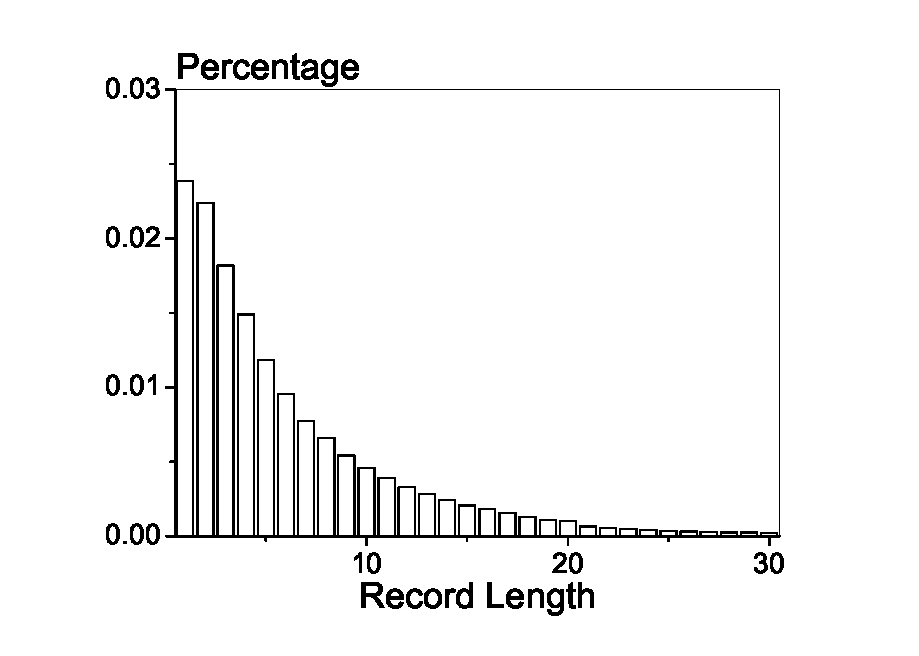
\includegraphics[width=1.0\columnwidth]{BMS-POS.eps}
\end{minipage}%
}
\subfigure[WV]{
\begin{minipage}[c]{0.46\textwidth}
  \includegraphics[width=1.0\columnwidth]{BMS-WEB.eps}
\end{minipage}%
}
\subfigure[Retail]{
\begin{minipage}[c]{0.46\textwidth}
  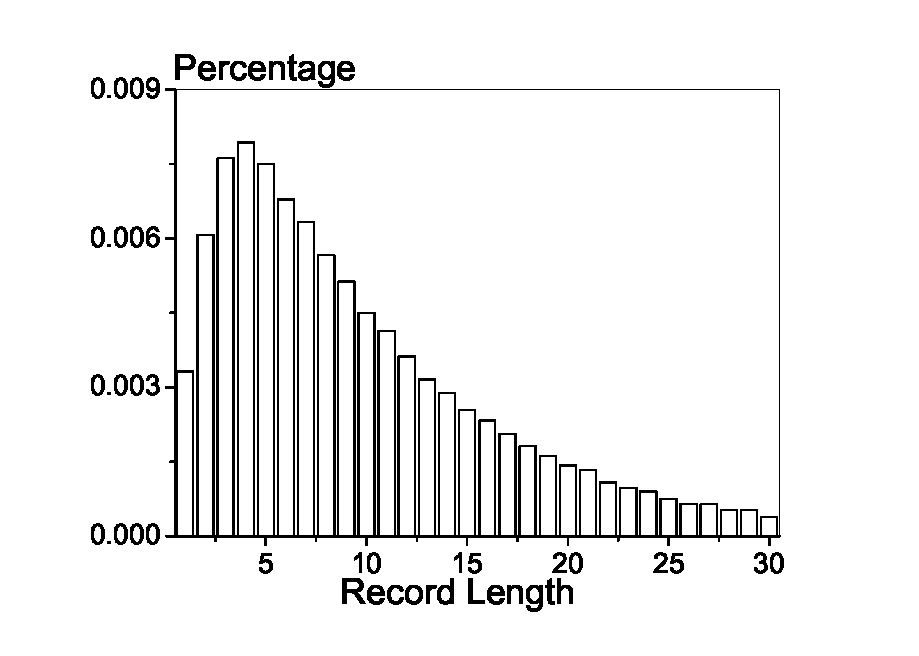
\includegraphics[width=1.0\columnwidth]{retail.eps}
\end{minipage}%
}
\subfigure[Syn]{
\begin{minipage}[c]{0.46\textwidth}
  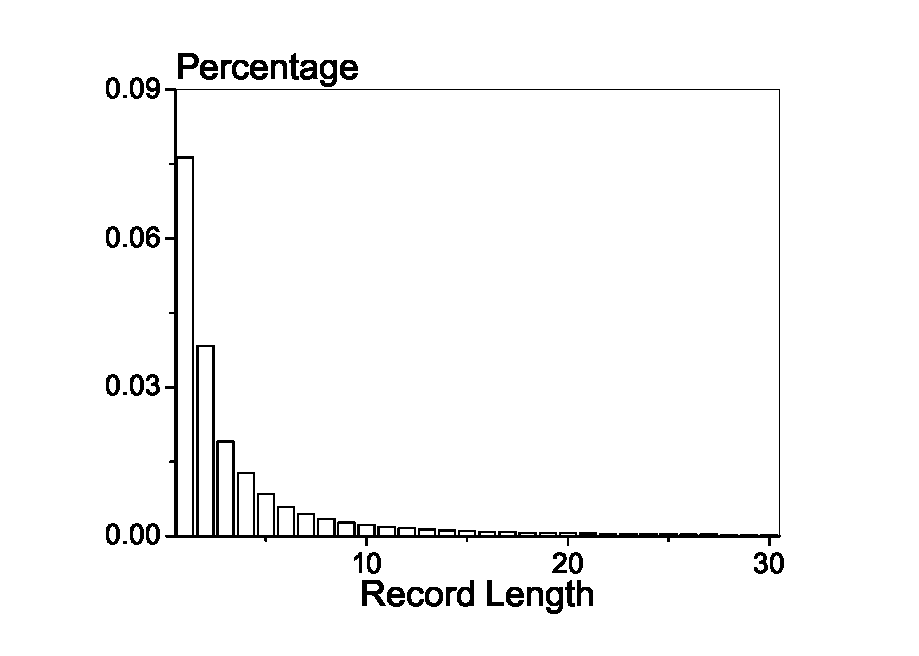
\includegraphics[width=1.0\columnwidth]{r50w.eps}
\end{minipage}%
}
\caption{Distribution in Record Length of Five Original Datasets}\label{fig:datasets}
\end{figure}


We compare our algorithm with the
global suppression algorithm (named Global) and generalization algorithm
(named TDControl) of
Cao {\em et al.} \cite{Cao:2010:rho}.\footnote{The source code of these
algorithms was directly obtained from Cao.}
%since these systems are most
%related to our work in terms of privacy model. In the rest of the section,
%by {\em Global} and {\em TDControl}, we mean these two algorithms.
Our algorithm has two variants, {\em Dist} and {\em Mine}, which optimize
for data distribution and rule mining, respectively.
%We also compare the performance of the above algorithms with a simple
%baseline algorithm denoted as {\em Random} which
%randomly picks one unsafe \qid and one item type in this \qid to suppress.
%In order to evaluate the ability to retain useful association rules and
%to avoid spurious rules in these competing algorithms, we need the ground
%truth, which are all the association rules inferrable from the datasets with
%sufficient confidence and support.
%However, original datasets are too large to infer all association rules.
Experiments that failed to complete in 2 hours is marked
as ``N/A'' or an empty place in the bar charts.
We run all the experiments on Linux 2.6.34)
with an Intel 16-core 2.4GHz CPU and 8GB RAM.
%Experiment programs are written in C++ and compiled using GCC version 4.5.0.

We design a metric, {\em info loss}, to evaluate how much information is lost after the partial compression.
\[\text{info loss} = \frac{{Items(T) - Items(T')}}{{Items(T)}}\]
Here, we define $Items(T)$ as the number of items in dataset $T$.
The method we adopt to calculate information loss is reasonable,
because ${Items(T) - Items(T')}$ represents the loss of raw data that
can be used for statistical analysis or association rule mining.
Obviously, {\em info loss} equals to 0 if there is no information loss.

\subsection{Variation of $\rho$}

\begin{figure}[tb]
\centering
\subfigure[Information Loss]{
\label{fig:rhoVar1}
\begin{minipage}[c]{0.45\textwidth}
\centering
  \includegraphics[width=7cm]{rhoil.eps}
\end{minipage}%
}
\subfigure[Data Distribution]{
\label{fig:rhoVar2}
\begin{minipage}[c]{0.45\textwidth}
\centering
  \includegraphics[width=7cm]{rhoKL.eps}
\end{minipage}%
}
\subfigure[Rule Mining]{
\label{fig:rhoVar3}
\begin{minipage}[c]{0.45\textwidth}
\centering
  \includegraphics[width=7cm]{jaccard.eps}
\end{minipage}%
}
\caption{Variation of $\rho$ (from 0 to 1)}\label{fig:rho}
\end{figure}

In this section, we gives the performance of our
algorithm with regard
to the variation of $\rho$.
To determine the similarity between the item frequency distribution
of original data and that of the anonymized data,
we use the Kullback-Leibler divergence (also called relative entropy) as our evaluation metric.
To prevent zero denominators, we modified \eqnref{eq:kl}
to a symmetric form \cite{Fisher:2008:DSF} defined as
\[\mathcal{S}(H_1||H_2)=\frac{1}{2}KL( H_1||H_1 \cup H_2)+\frac{1}{2} KL( H_2||H_1 \cup H_2)\]
where  $H_1 \cup H_2$ represents the union of distributions $H_1$ and $H_2$.
We take WV as our test data.
Figure \ref{fig:rhoVar1} shows that
the information loss decreases when $\rho$ becomes larger.
The reason is clear: as $\rho$ grows,
there are fewer unsafe qids in the data and
fewer suppressions need to be executed and hence less information
loss. Figure \ref{fig:rhoVar2} shows that data distribution
is better when $\rho$ becomes larger.
The reason should also be attributed to
the fewer suppressions executed when $\rho$ becomes larger. Fewer suppressions mean
less disturbance to the original distribution.
Figure \ref{fig:rhoVar3} shows the relation between $\rho$ and the Jaccard Similarity of $R(T)$ and $R(T')$. It is
an interesting curve that initially rises slowly with $\rho$,
but then drops drammatically. Our explanation is,
when $\rho$ is relatively small, Jaccard Similarity increases with $\rho$ because fewer suppressions lead to
fewer original rules deleted and fewer spurious rules added. When $\rho$ becomes relatively large,
the descendence of Jaccard Similarity should be attributed to the shrinkage of the sizes of $R(T)$ and $R(T')$.
When $\rho$ is relatively large, it is hard to mine association rules from dataset so the size of ruleset is small.
And it is natural that when the sizes of both sets are comparatively small, it is difficult for them to be similar.
When $\rho$ is 0.9, we find no association rule in the suppressed dataset and only 1 rule in the
original dataset. Therefore, the Jaccard Similarity is 0.
\footnote{When we do rule mining, we adopt the A-priori algorithm and set the minimum support rate to be
$0.05\%$, which is a reasonable value in practice.}

In what follows, we first present results in data utility, then the
performance of the algorithms, and then the effects of
changing various parameters in our algorithm.
Finally, we compare with a permutation method which utilizes
a similar privacy model but with different optimization goals.
Based on previous observations, we choose two representative values of $\rho$,
$0.3$ and $0.7$, for the data utility experiments, and $\rho=0.7$ for other experiments.
Unless otherwise noted, we use the following default parameters:
$b_{max} = 10^6$, $t_{max}=500$. These default
parameters are carefully set to provide better results
and to ensure that the process can terminate in a reasonable
amount of time.
For example, we set $b_{max} = 10^6$ for it can provide a buffer
big enough to hold all $qid$s. If we use a smaller one,
the execution time will be lengthened to be reloading of buffer
space. Also, we set $b_{max} = 10^6$ because $log_2(10^6) \approx 20$, 
which bounds the average record length of our data sets.
Such practice balances $b_{max}$ and ${2^{\frac{N}{|T|}}}$ 
in \eqnref{eq:complexity}.
If $b_{max}$ is too large, it will result in waste of
space. We set $t_{max} = 500$ since it is an appropriate time
for the execution of each divide-and-conquer problem.

\subsection{Data Utility}\label{sec:eval:datautility}
We compare the algorithms in terms of information loss, data distribution,
and association rule mining. As TDControl generates rules in general form,
we adopt a specialization method for the evaluation of its information loss,
which we will explain at the end of section 4.2.

\begin{figure}[tb]
\centering
\subfigure[ $\rho=0.3$]{\label{fig:loss-a}
\hspace{-1cm}
\begin{minipage}[c]{0.45\textwidth}
  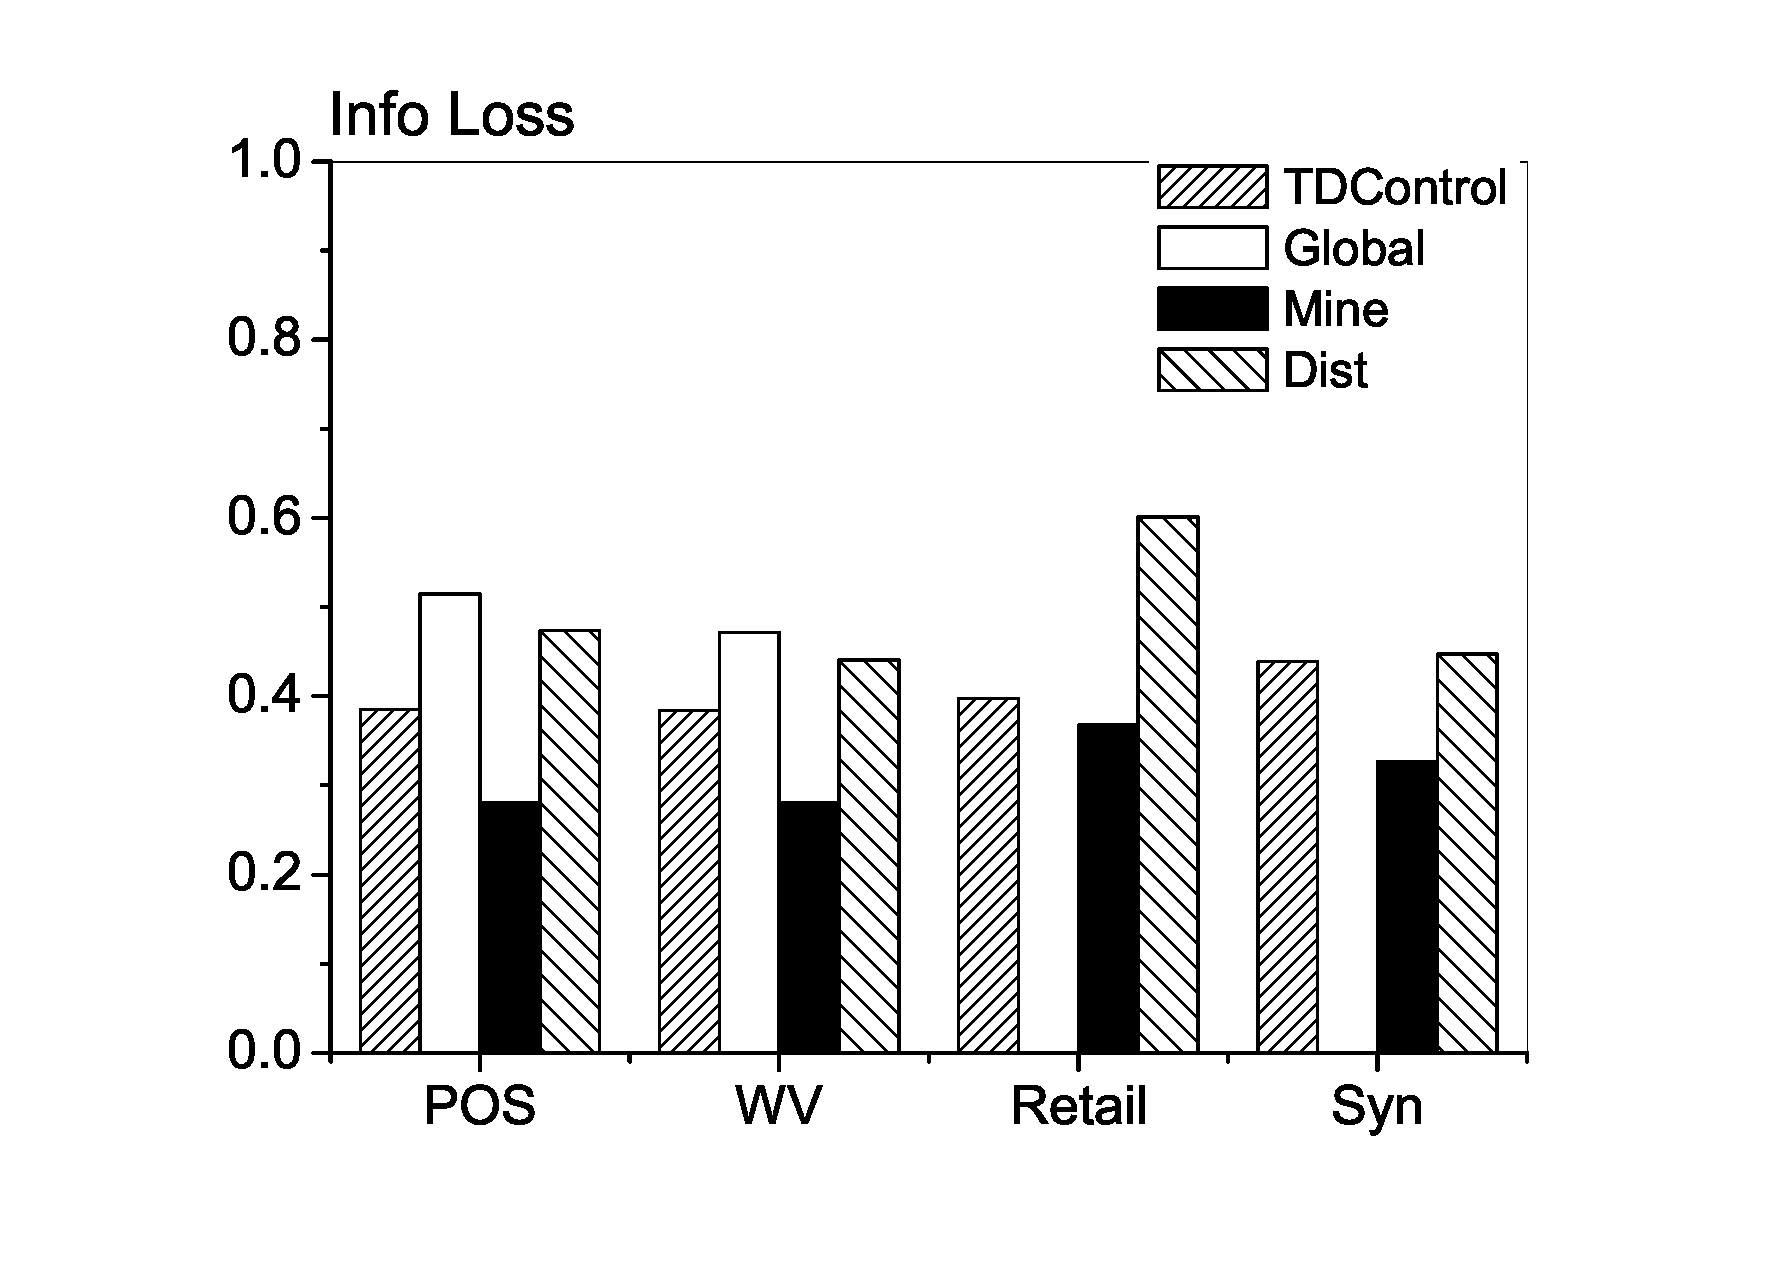
\includegraphics[width=7cm]{loss3.eps}
\end{minipage}%
}
\subfigure[ $\rho=0.7$]{\label{fig:loss-b}
\begin{minipage}[c]{0.45\textwidth}
  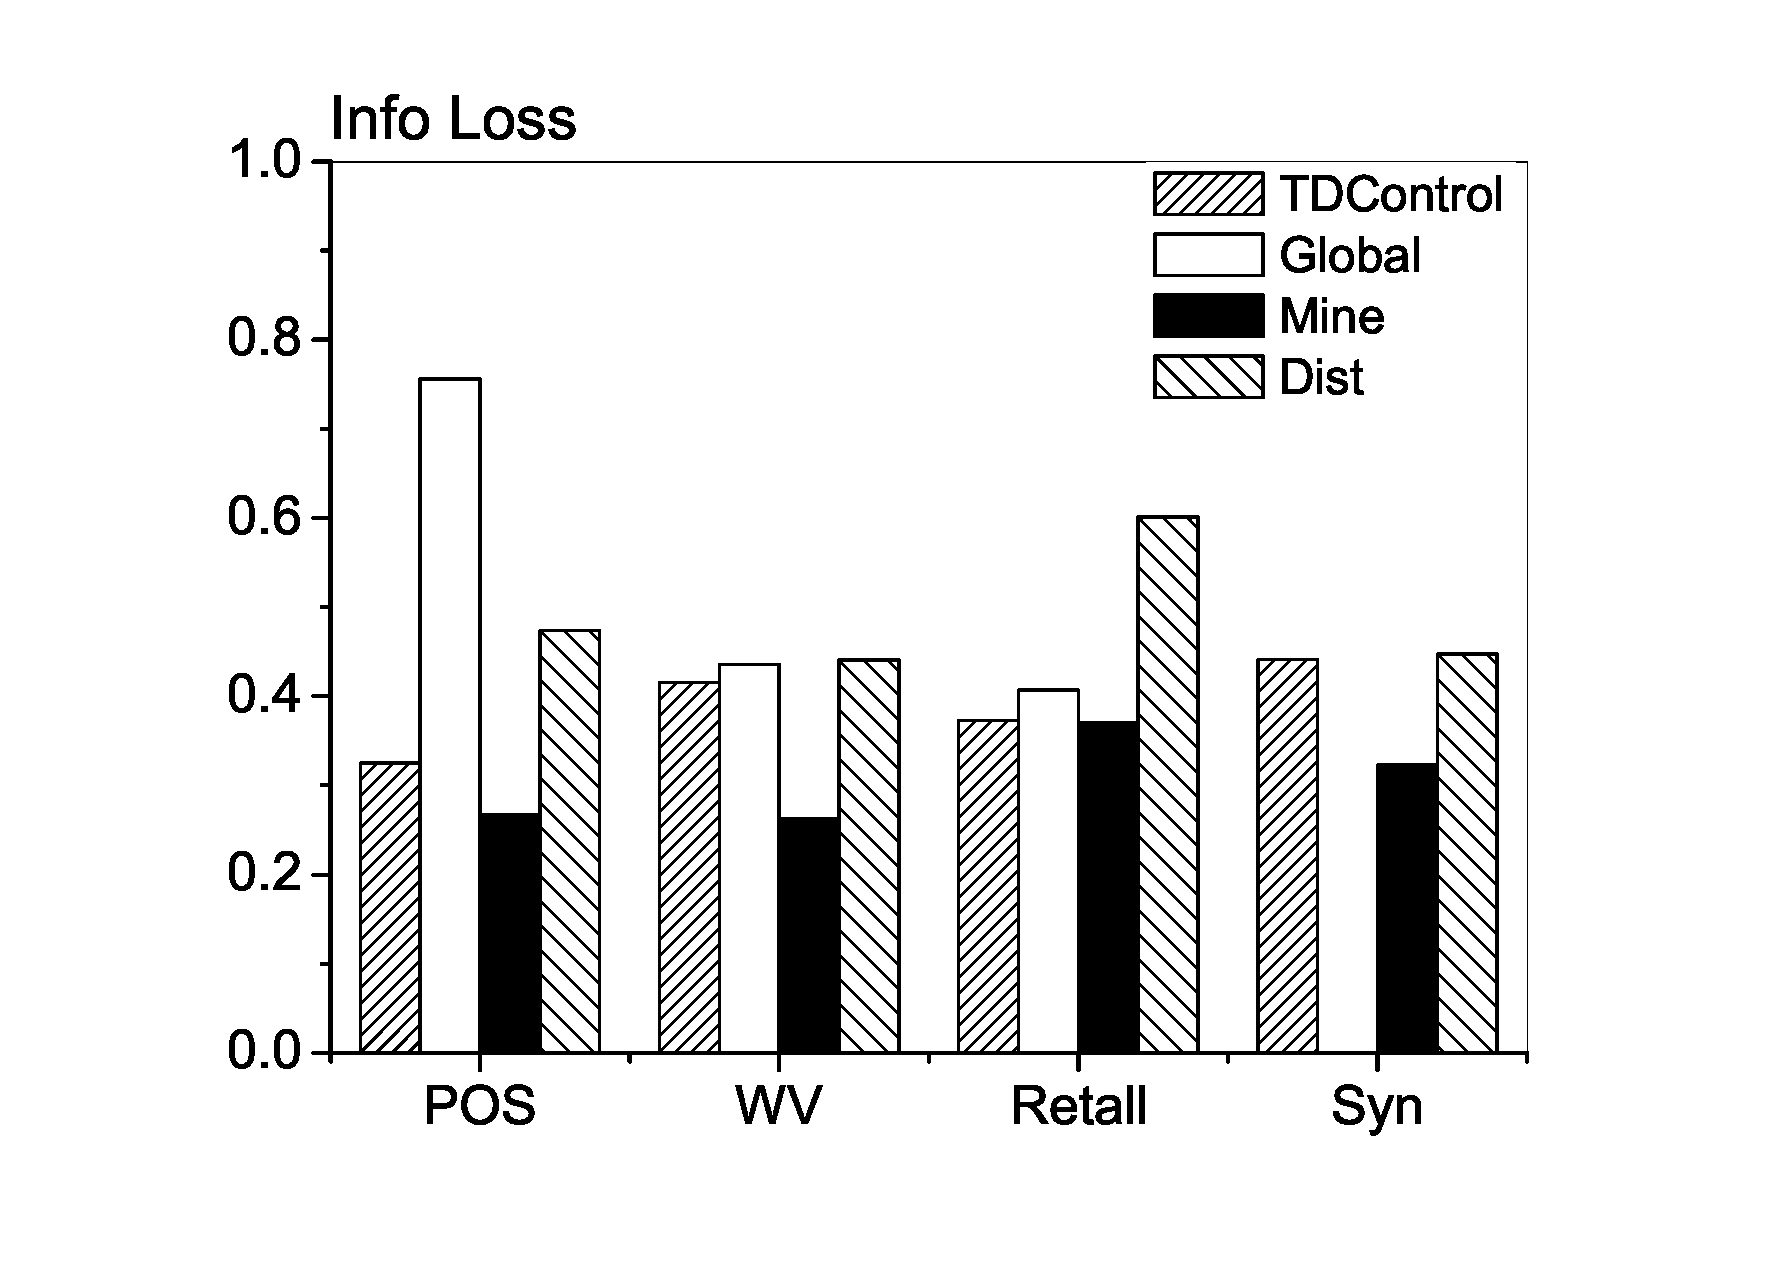
\includegraphics[width=7cm]{loss7.eps}
\end{minipage}%
}
\subfigure[different $\rho$]{\label{fig:loss-c}
\begin{minipage}[c]{0.45\textwidth}
\centering
  \includegraphics[width=7cm]{infoloss.eps}
\end{minipage}%
}
\caption{Comparisons in Information Loss}\label{fig:loss}
\end{figure}

Figure \ref{fig:loss}
shows that $Mine$ is uniformly better among the four techniques.
It suppresses only about 26\% items in POS and WV and about 35\% items in
Retail, while the other three techniques incur on average 10\% more losses
than  $Mine$ and up to 75\% losses in the worst case. We notice that $Dist$
has a generally worse performance than other techniques even though it tries to minimize the
information loss at each iteration.
The reason is that it also tries to retain the data
distribution.
%We will see how this heuristic works in retaining the data
%distribution in Section \ref{sec:eval:datadistribution}.
Further, we argue that for applications that require data statistics,
the distribution, that is, the summary information, is more useful than the
details, hence losing some detailed information is acceptable.
Note that Global and TDControl failed to complete in some datasets,
because these methods don't scale very well.
%This confirms that our alogrithm causes less information losses than peers.
%which suggests that our algorithm scales better on bigger data than the
%existing approaches.
%indicating that our algorithm has a
%strong flexibility in $\rho$.
%\subsubsection{Data Distribution}\label{sec:eval:datadistribution}

\begin{figure}[tb]
\centering
\subfigure[ $\rho=0.3$]{
\hspace{-1cm}
\begin{minipage}[c]{0.45\textwidth}
\centering
  \includegraphics[width=7cm]{relative3.eps}
\end{minipage}%
}
\subfigure[ $\rho=0.7$]{
\begin{minipage}[c]{0.45\textwidth}
\centering
  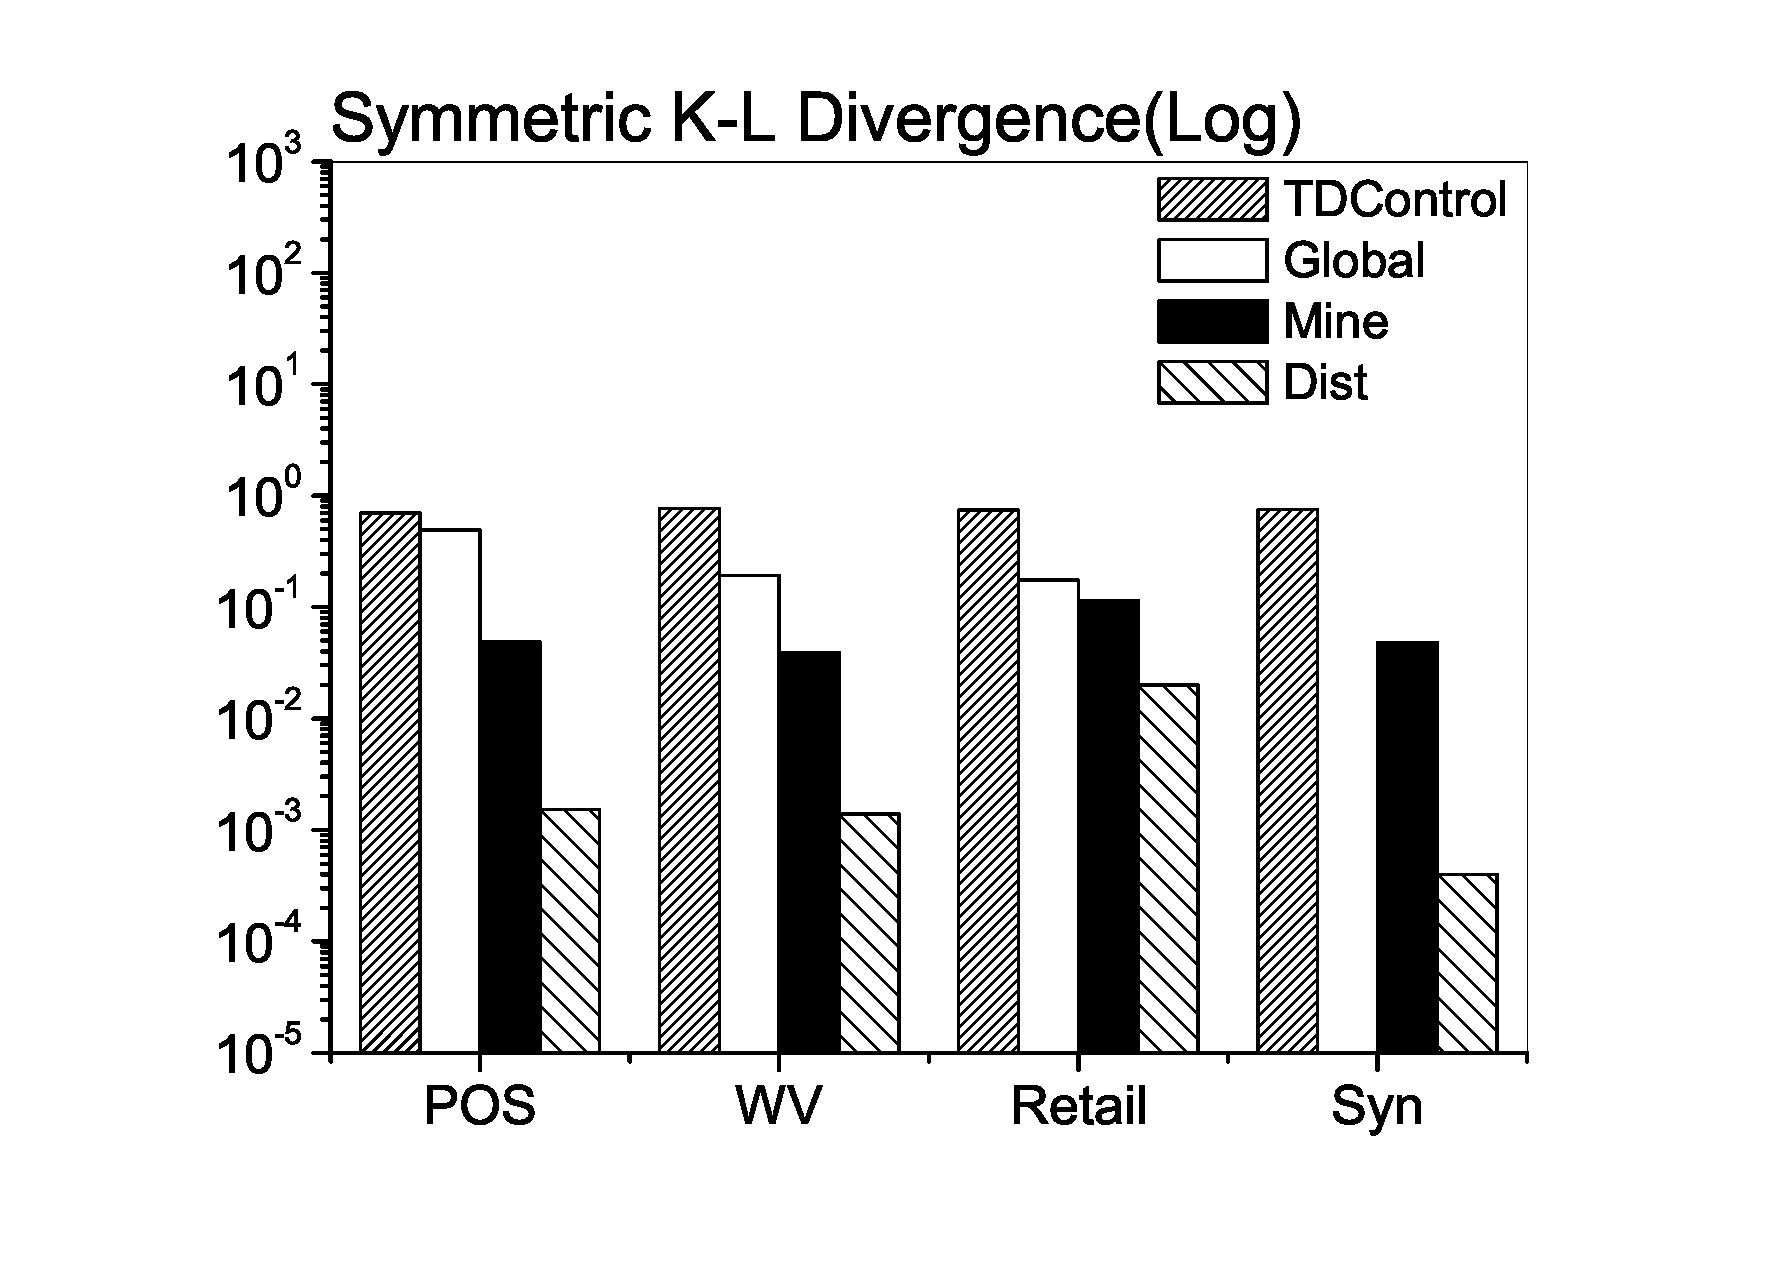
\includegraphics[width=7cm]{relative7.eps}
\end{minipage}%
}
\subfigure[ different $\rho$]{
\begin{minipage}[c]{0.45\textwidth}
\centering
  \includegraphics[width=7cm]{KL.eps}
\end{minipage}%
}
\caption{Comparisons in Symmetric K-L Divergence}
\label{fig:entropy}
\end{figure}

Figure \ref{fig:entropy} shows that $Dist$ outperforms the peers
 as its output has the highest resemblance
to the original datasets.
On the contrary, TDControl is the worst performer
since generalization algorithm creates a lot of new items while
suppressing too many item types globally.
Since the symmetric relative entropy of $Dist$ is very small, y-axis is
in logrithmic scale to improve visibility. Therefore, the actual difference
in K-L divergence is two to three orders of magnitude.
The most common criticism of partial suppression is that it
changes the support of good rules in the data and introduces spurious
rules in rule mining. In this experiment, we test the algorithms on
data sets with the max record length=5 (cutoff=5),
and check the rules mined from the anonymized data
with minimum support rate equal to
0.05\% \footnote{We choose this support level just to
reflect a practical scenario.}.
%Mining rules from the original datasets with many
%long records is prohibitive due to large memory requirements.
Figure \ref{fig:rulemining1},\ref{fig:rulemining2} gives the performance of different anonymization methods.
Both TDControl and Global perform badly in this category, with
negligible number of original rules remaining after anonymization.
Conversely, all of the partial
suppression algorithms manage to retain most of the rules and the Jaccard Similarity reaches 80\% in some datasets which shows
our heuristic works very well.
Specifically, $Mine$ performs the best among partial algorithms.

The rules generated from TDControl are all in general form which is
totally different from the original one. To enable comparison,
we specialize the more general rules from the result of TDControl
into rules of original level of abstraction in the generalization hierarchy.
For example, we can specialize a rule \{dairy product $\rightarrow$ grains\}
into:
\rm{milk} $\rightarrow$ \rm{wheat},
\rm{milk} $\rightarrow$ \rm{rice},
\rm{yogurt} $\rightarrow$ \rm{wheat}, etc.
%\rm{yogurt} $\rightarrow$ \rm{rice}\\
Take WV as an example, there are 4 rules left in the result of TDControl when
the $\rho$ is 0.7 and the number becomes 28673 after
specialization, which makes the results almost invisibly short
on the figures.

Figure \ref{fig:rulemining3} shows the trend of Jaccard Similarity when $\rho$ varies using partial suppression.
We present the results of datasets POS(cutoff=5) and WV(cutoff=5) in the figure.
Datasets Retail(cutoff=5) and Syn(cutoff=5) fail to complete within 2 hours, so we leave them out.
We can see that Jaccard Similarity generally increases as $\rho$ grows larger.
But when $\rho$ is relatively large, the Jaccard Similarity curve
exhibits some anomaly. It is because
the size of ruleset is small when $\rho$ is relatively large,
and Jaccard Similarity does not work very well to assess
the similarity of two very small sets.
The differences in datasets will have a significant impact on
Jaccard Similarity when $\rho$ is
relatively large.
For example, when $\rho=0.9$,
there is one rule left in the rulesets mined from
original data and suppressed data by {\em POS-dist}, and
these two rules happen to be the same.
Consequently the Jaccard Similarity is as high as 1.
\begin{figure}[tb]
\centering
\subfigure[ $\rho=0.3$]{
\label{fig:rulemining1}
\hspace{-1cm}
\begin{minipage}[c]{0.45\textwidth}
\centering
   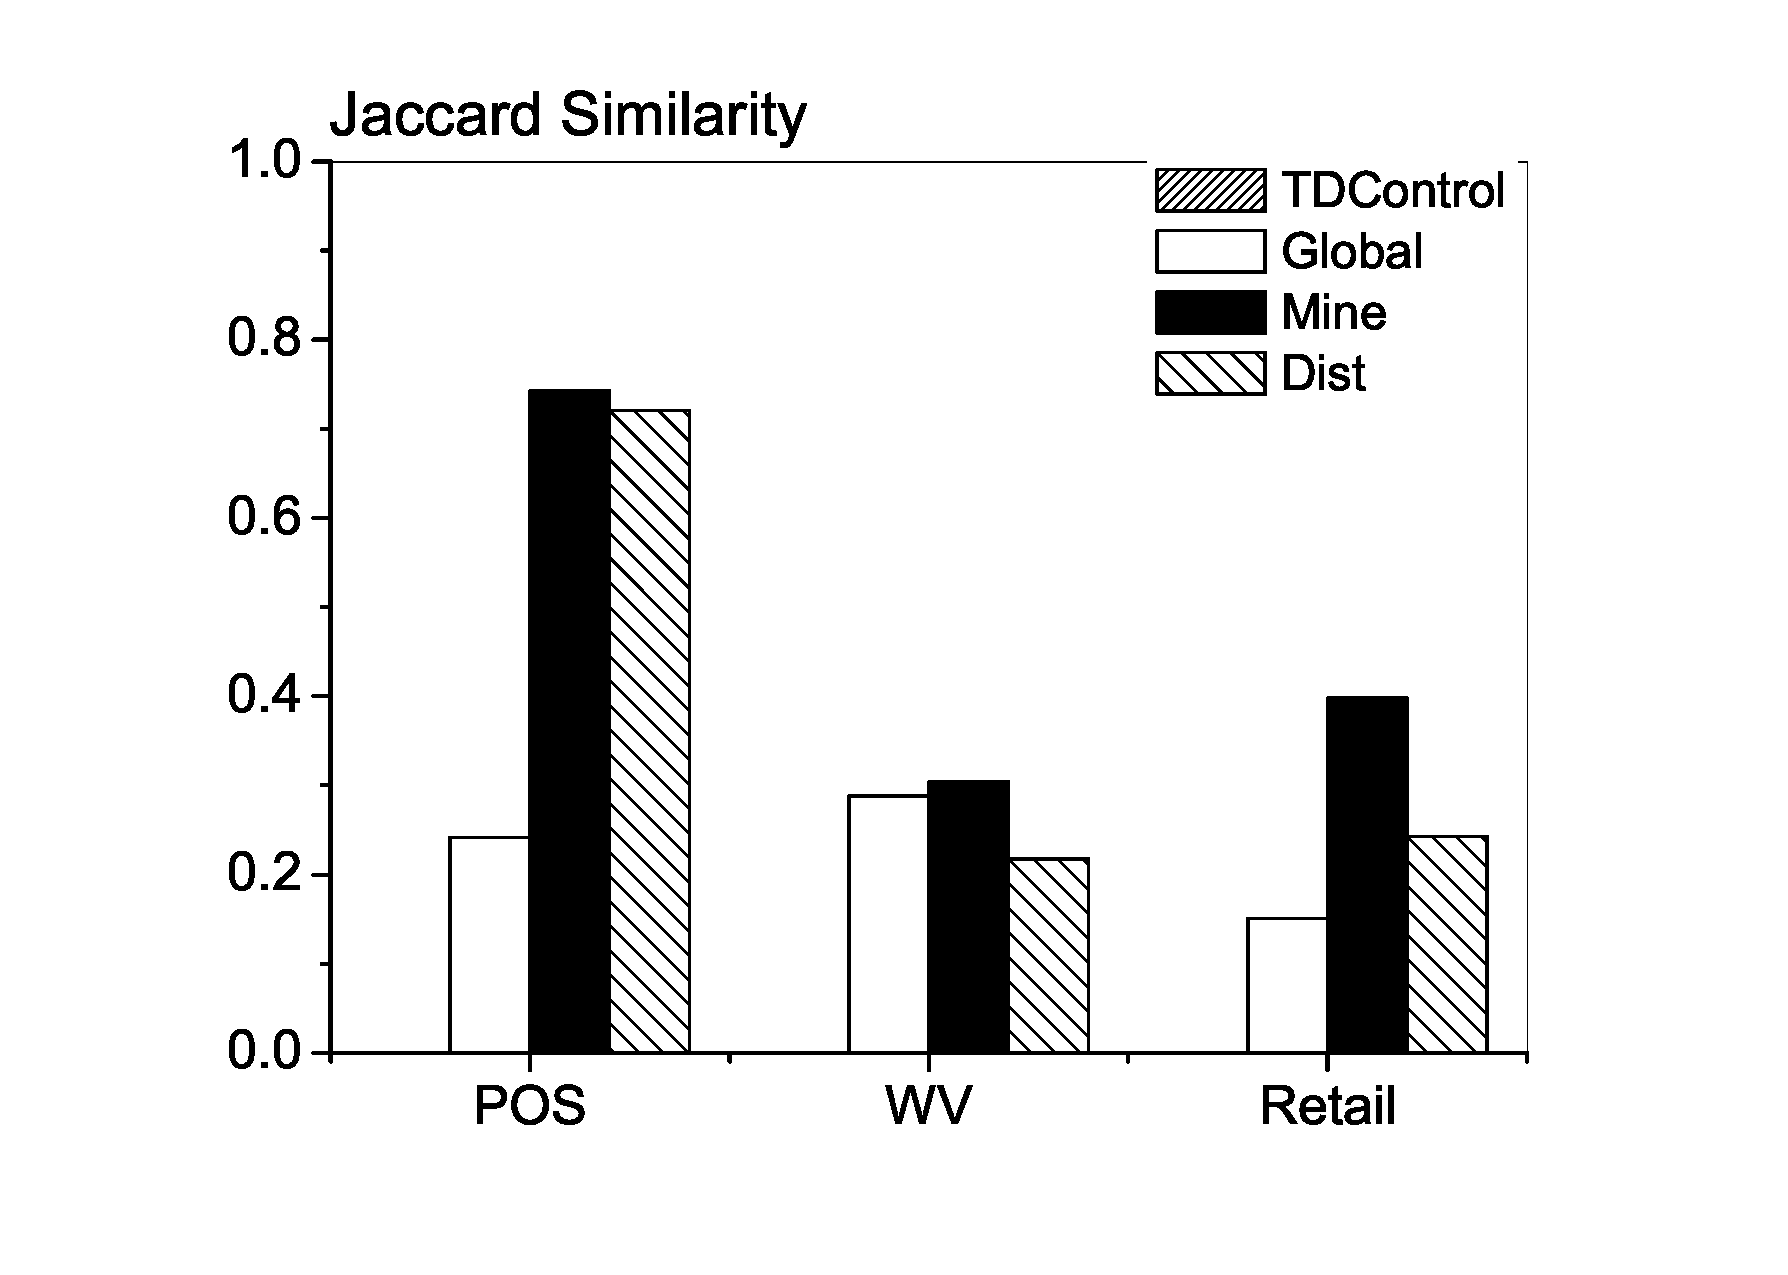
\includegraphics[width=7cm]{js3.eps}\\
\end{minipage}%
}
\subfigure[ $\rho=0.7$]{
\label{fig:rulemining2}
\begin{minipage}[c]{0.45\textwidth}
\centering
  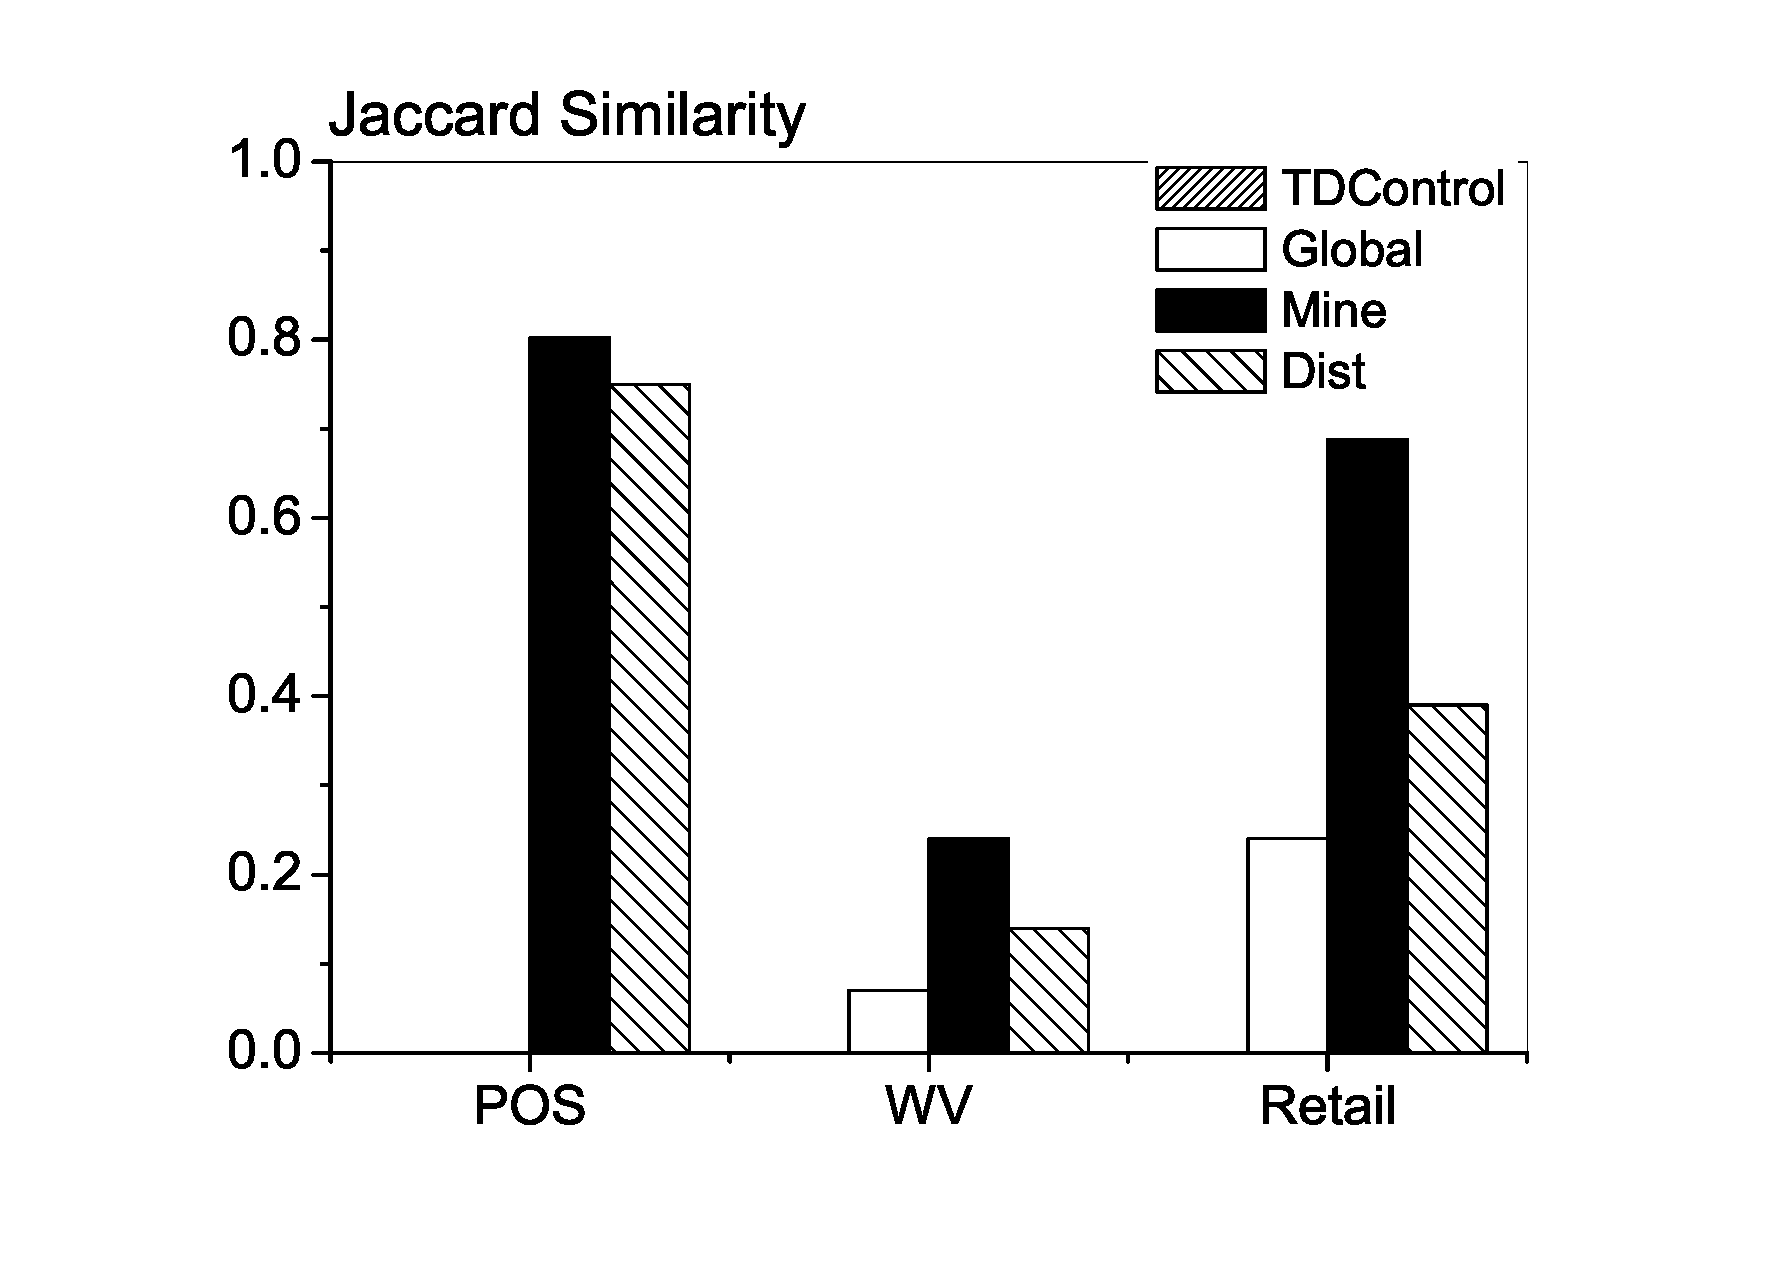
\includegraphics[width=7cm]{js7.eps}
\end{minipage}%
}
\subfigure[ different $\rho$]{
\label{fig:rulemining3}
\begin{minipage}[c]{0.45\textwidth}
\centering
  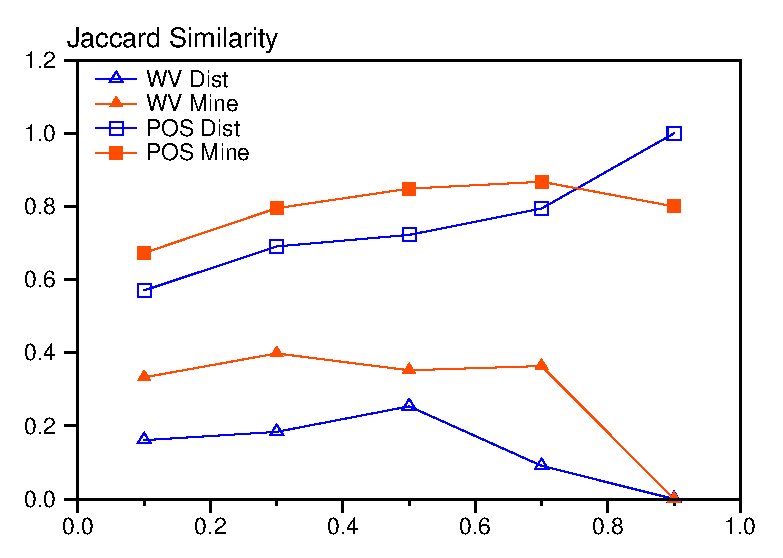
\includegraphics[width=7cm]{J.eps}
\end{minipage}%
}
 \caption{Association Rules Mining with Support $0.05 \%$}
 \label{fig:rulemining}
\end{figure}

\subsection{Performance}\label{sec:eval:performance}
Next we evaluate the time performance and scalability of
our algorithms.

%\subsubsection{Time Performance}\label{sec:eval:time}
\begin{table}[bh]
\caption{Comparison in Time Performance ($\rho=0.7$, $t_{max}=300$)
\label{tab:timeresult}}
\centering
\begin{tabular}{|l|r|r|r|r|r|}
  \hline
  % after \\: \hline or \cline{col1-col2} \cline{col3-col4} ...
  Algorithm & POS & WV & Retail  &Syn \\  \hline \hline
  TDControl & \bf{183} & \bf{30 }& \bf{156} &   476  \\  \hline
  Global & 1027 & 81 & 646 &   N/A  \\  \hline
%  \PartialR & 6582 & 305 & 1497 & 323&761 \\\hline
 % $Random$ & 814 & 188 & \bf{151} & \bf{105} \\\hline
  $Dist$ & 395 & 151 & 171 &\bf{130}\\ \hline
  $Mine$ & 1554 & 478& 256 & 132\\ \hline
  \end{tabular}
\end{table}

%Since data anonymization often takes place in offline mode,
%time performance is often not critical.
%Nonetheless, time matters if we want our algorithm to
%scale to large datasets.
%But reasonable time performance is still important for a data user.
From Table \ref{tab:timeresult}, TDControl is the clear winner
for two of the four datasets. $Mine$ does not perform well in BMS-POS.
The reason is that $Mine$ incurs the least information loss among all the
competiting methods. This means most of the original data remains
unsuppressed. Given the large scale of BMS-POS, checking whether the
dataset is safe in each iteration is therefore more time consuming than
other methods or in other datasets.
Results for Global are not available for Syn because
it runs out of memory.

%\subsubsection{Scalability}\label{sec:eval:scale}
Next experiment illustrates the scalability of our algorithm
w.r.t. data size. We choose $Retail$ as our target dataset here
%since the number of \qids increases dramatically with
%the increase of the records length
because $Retail$ has the maximum average record length of 10.6.
We run partial algorithms on 1/5, 2/5 through 5/5 of $Retail$ respectively.
Figure \ref{fig:scale} shows
the time cost of our algorithm increases reasonably with the
input data size with or without DnC.
%On Retail with DnC, data is partitioned into
%two pieces at 2/5 data, four pieces at 3/5 and 4/5 data, and then
%eight pieces for the whole data.
Furthermore, increased level of partitioning causes the algorithm to witness
superlinear speedup in Figure \ref{fig:scale:a}. In particular, the dataset is
automatically divided into 4, 8, 16 and 32 parts at 1/5, 2/5, 3/5 and
the whole of the data, respectively.
\begin{figure}[tb]
\centering
\subfigure[With DnC]{\label{fig:scale:a}
\hspace{-1cm}
\begin{minipage}[c]{0.45\textwidth}
\centering
  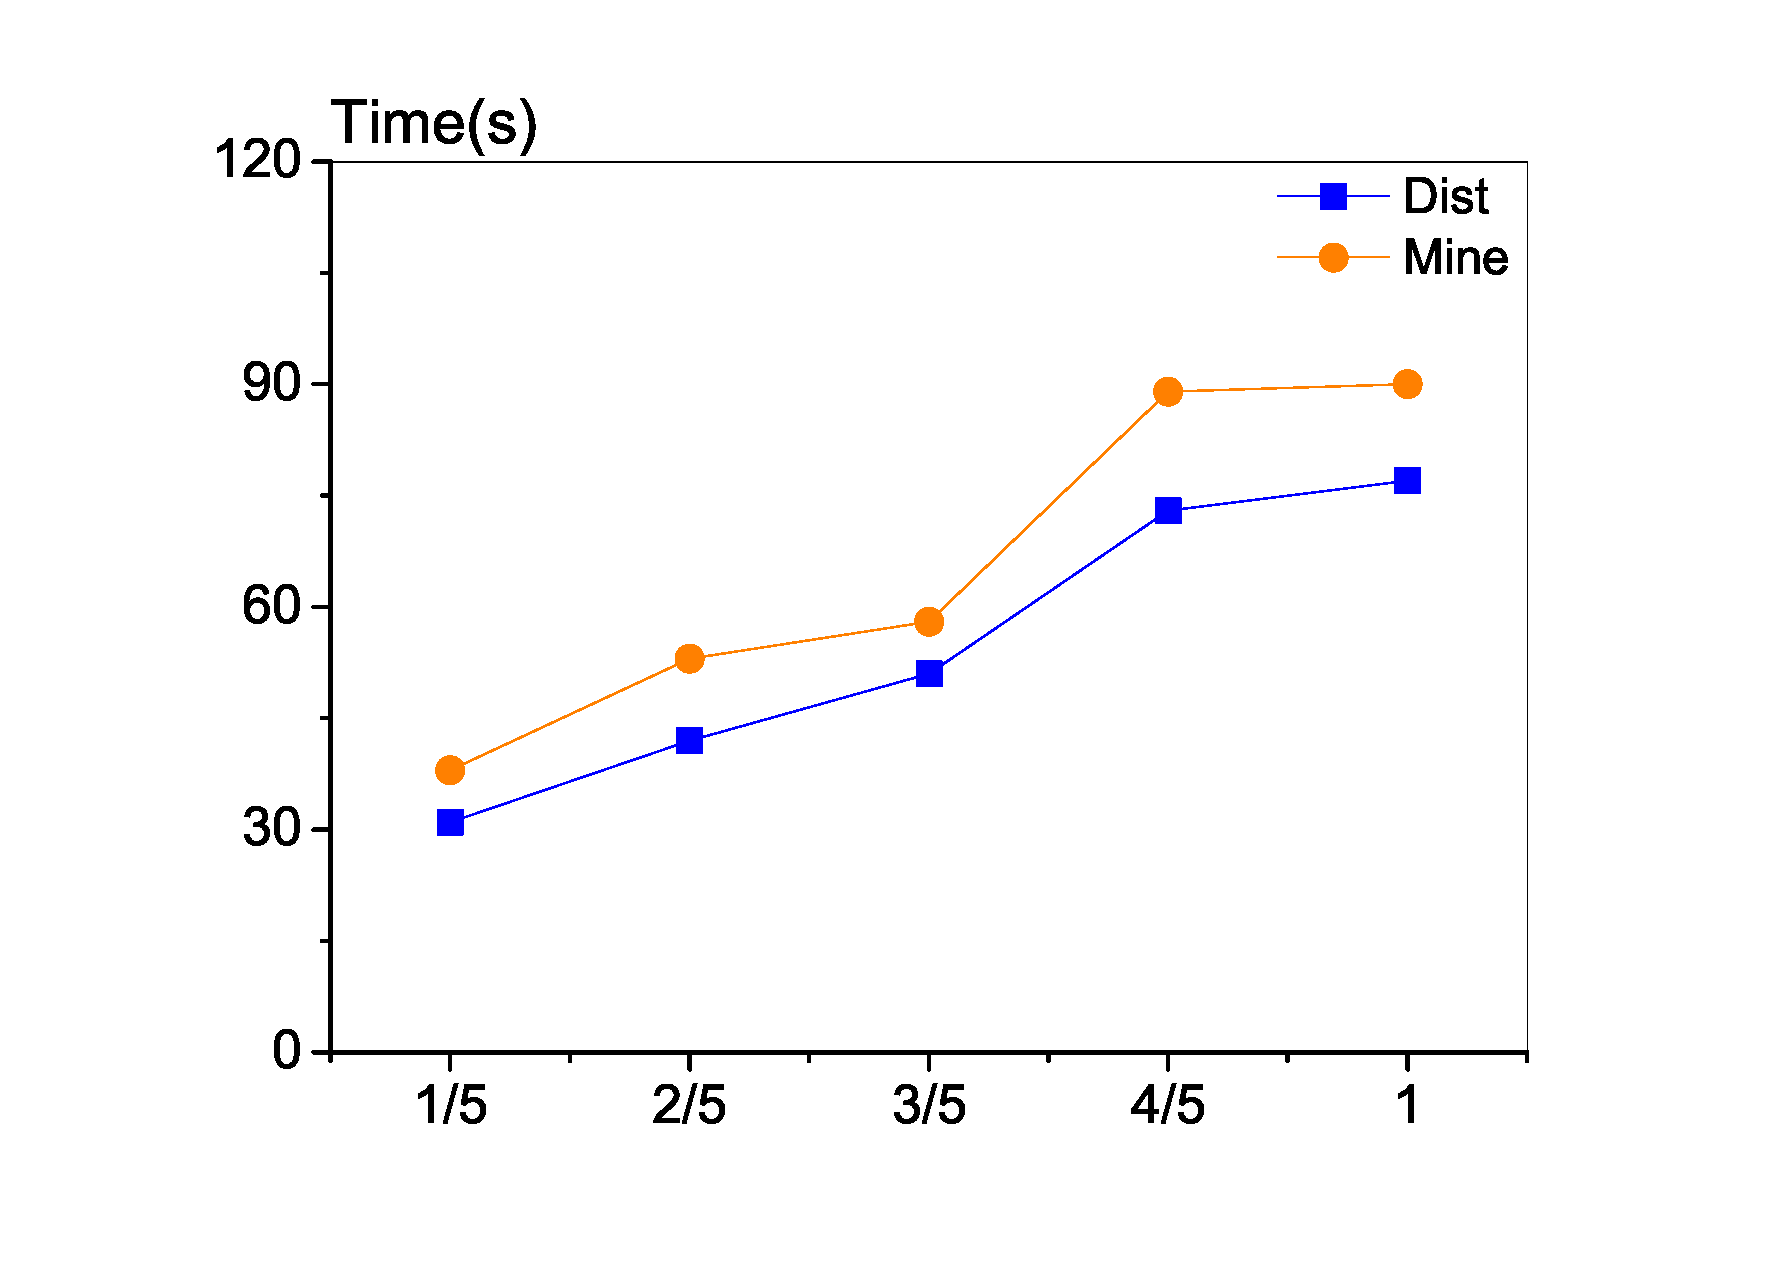
\includegraphics[width=7cm]{scaletime.eps}
\end{minipage}%
}
\subfigure[Without DnC]{\label{fig:scale:b}
\begin{minipage}[c]{0.45\textwidth}
\centering
  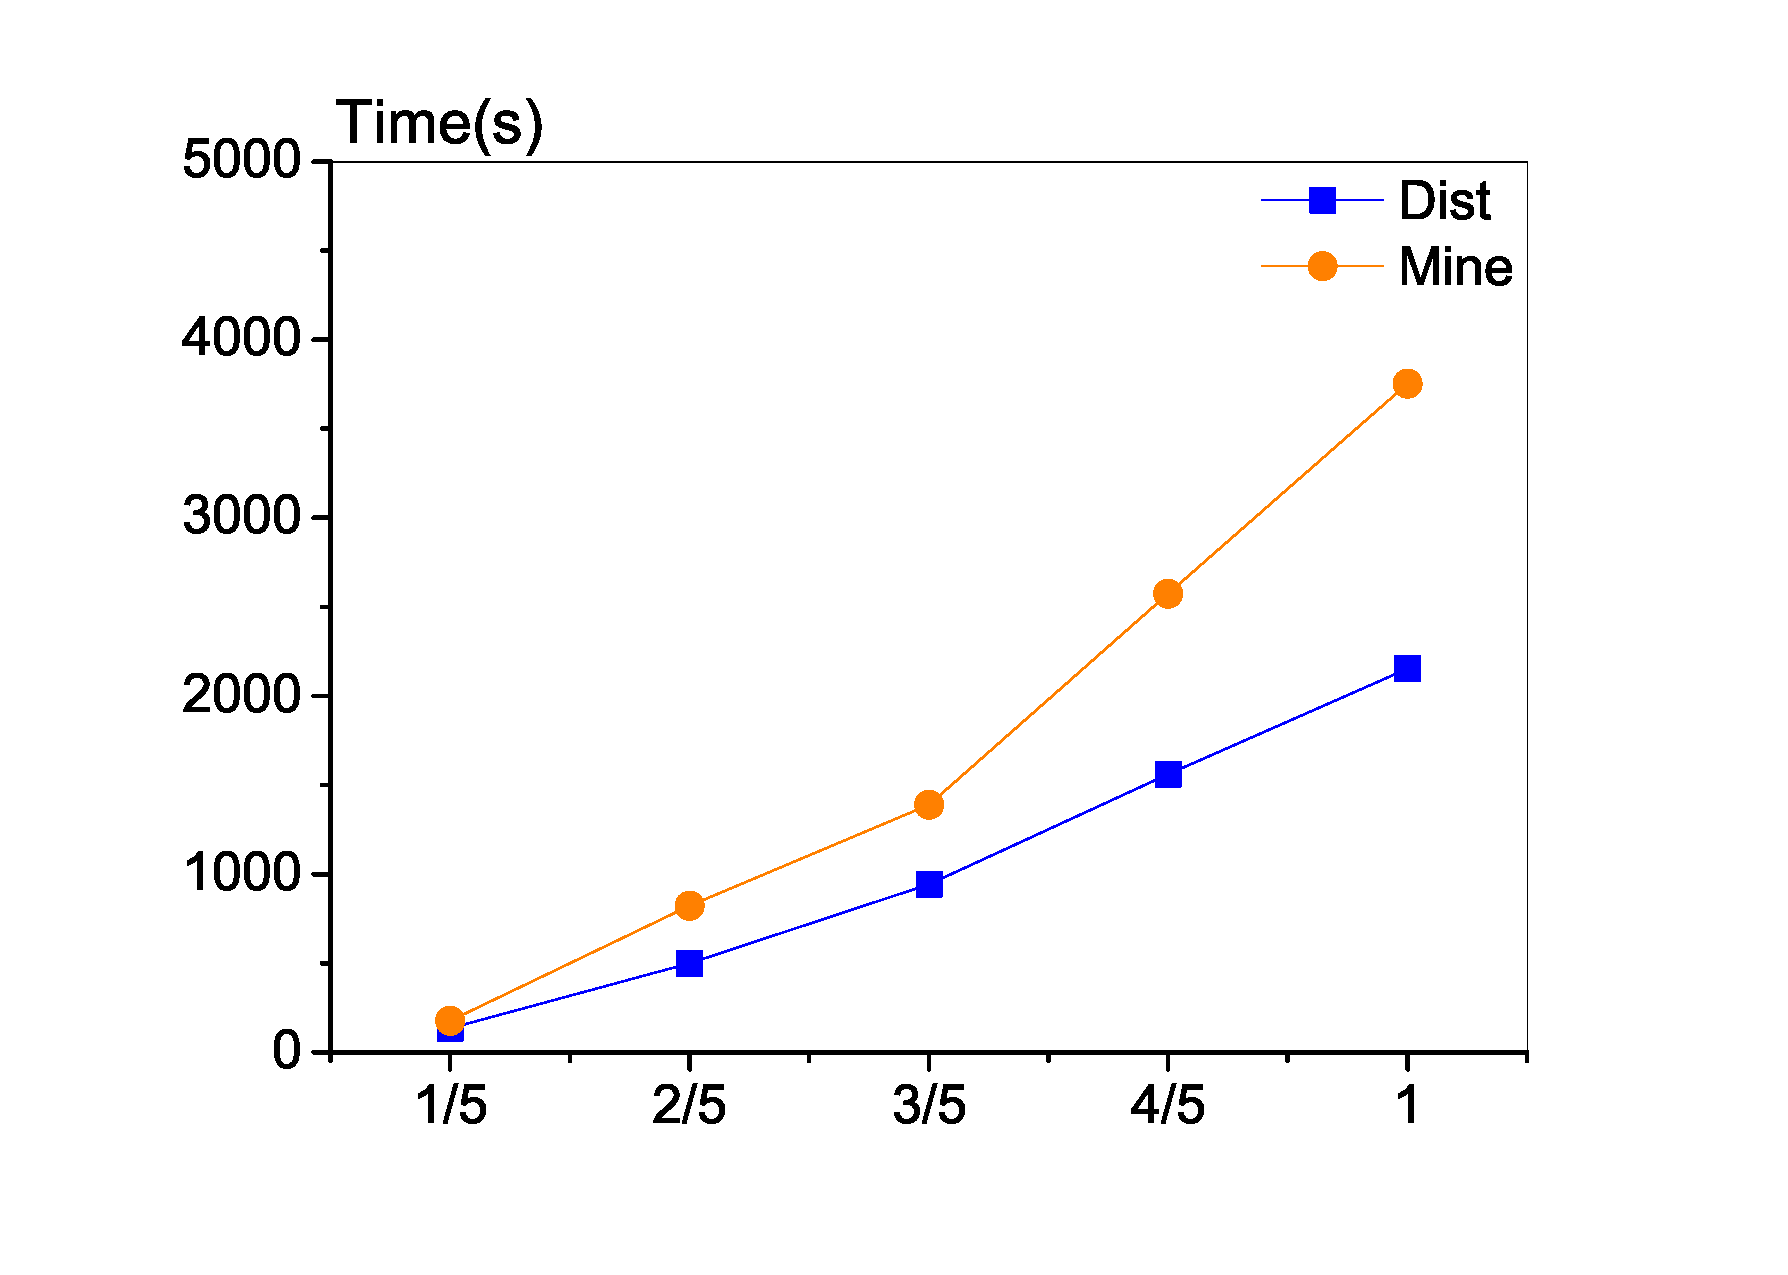
\includegraphics[width=7cm]{scaletimeno.eps}
\end{minipage}%
}
\caption{Scale-up with Input Data ($\rho=0.7$)}\label{fig:scale}
\end{figure}

\subsection{Effects of Parameters on Performance}\label{sec:eval:effect}
In this section,
we study the effects of $t_{max}$, $b_{max}$ on the
quality of solution (in terms of information loss) and time performance.

\subsubsection{Variation of $t_{max}$}\label{sec:eval:timebound}

%timebound
\begin{figure}[tb]
\centering
\subfigure[Information Loss]{
\label{fig:timebound-a}
\hspace{-1cm}
\begin{minipage}[c]{0.45\textwidth}
\centering
  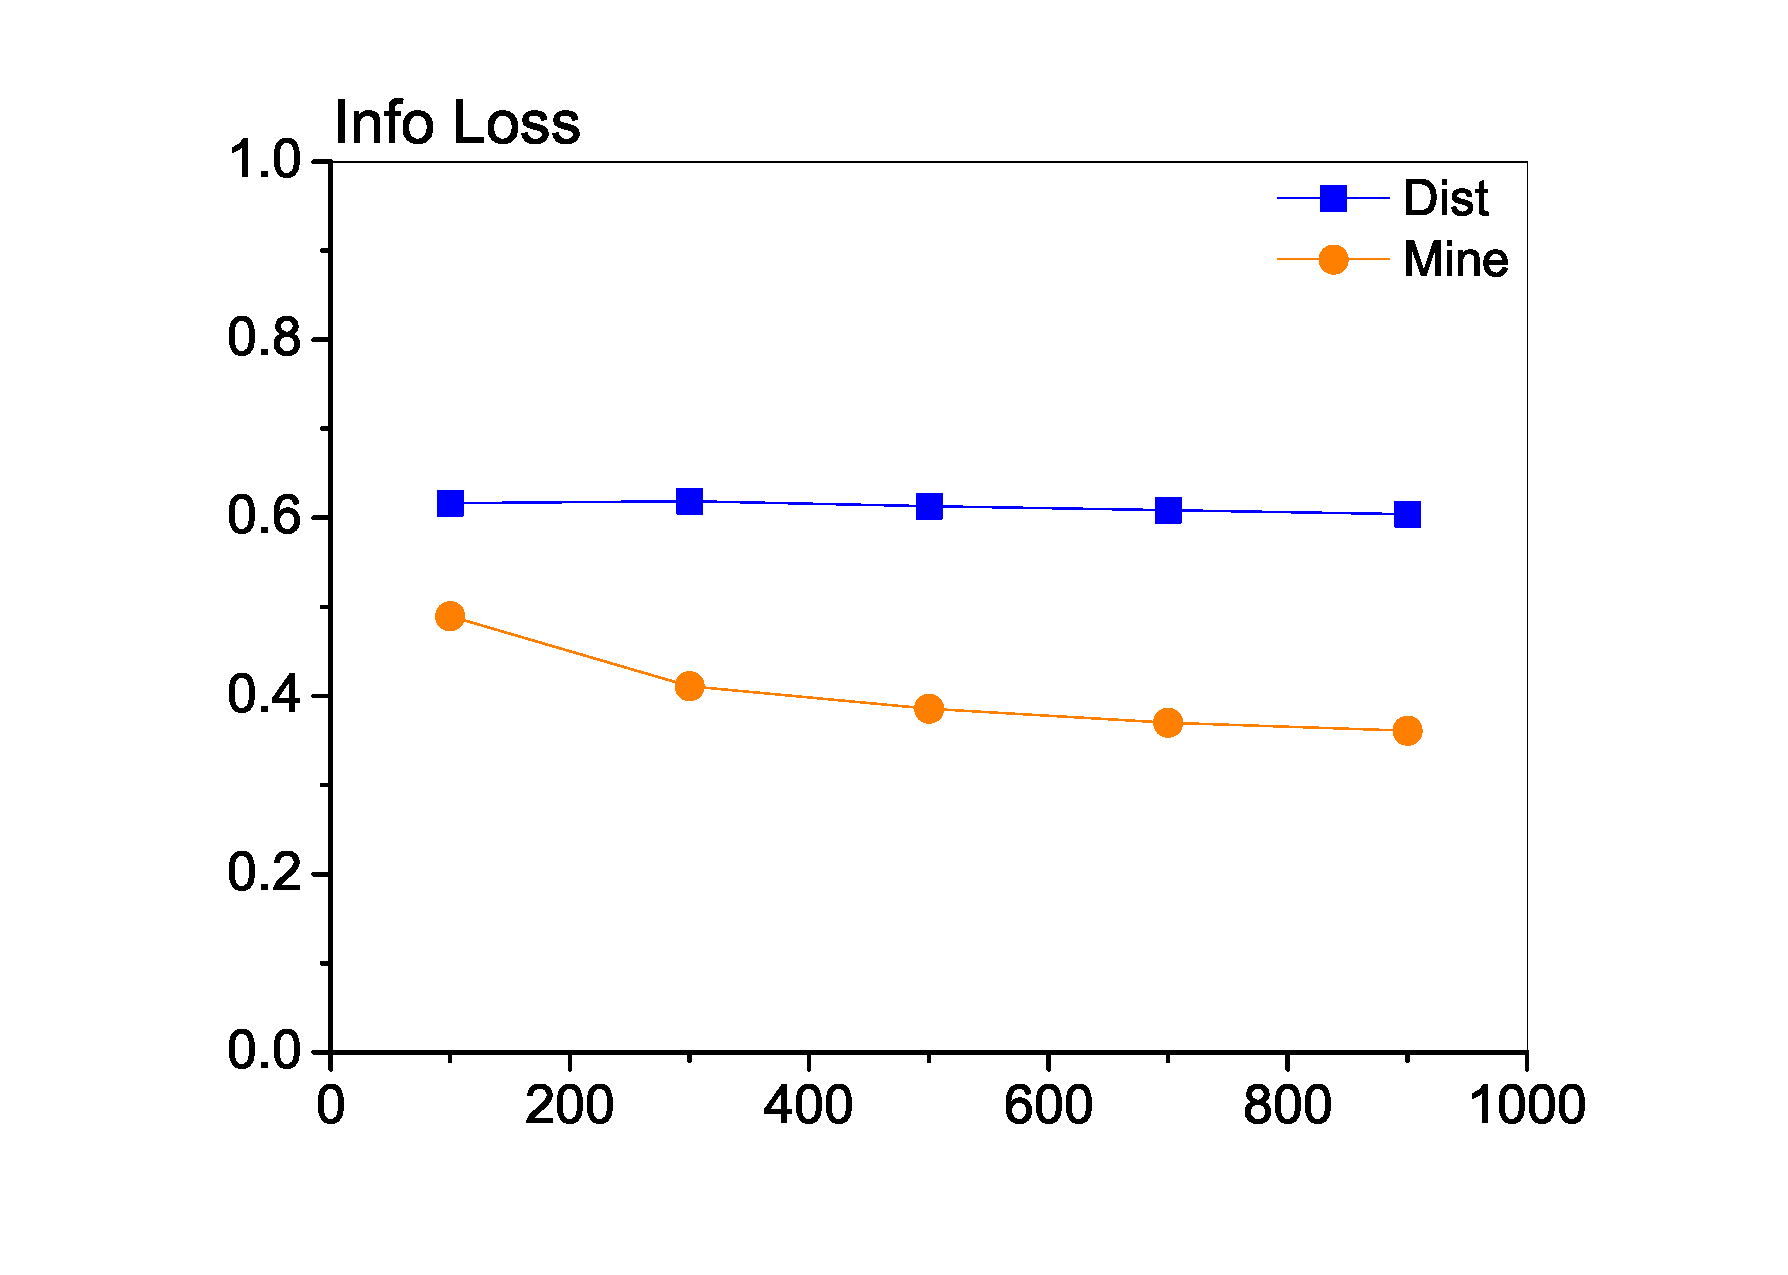
\includegraphics[width=7cm]{timebond_avg.eps}
\end{minipage}%
}
\subfigure[Time Performance]{
\label{fig:timebound-b}
\begin{minipage}[c]{0.45\textwidth}
\centering
  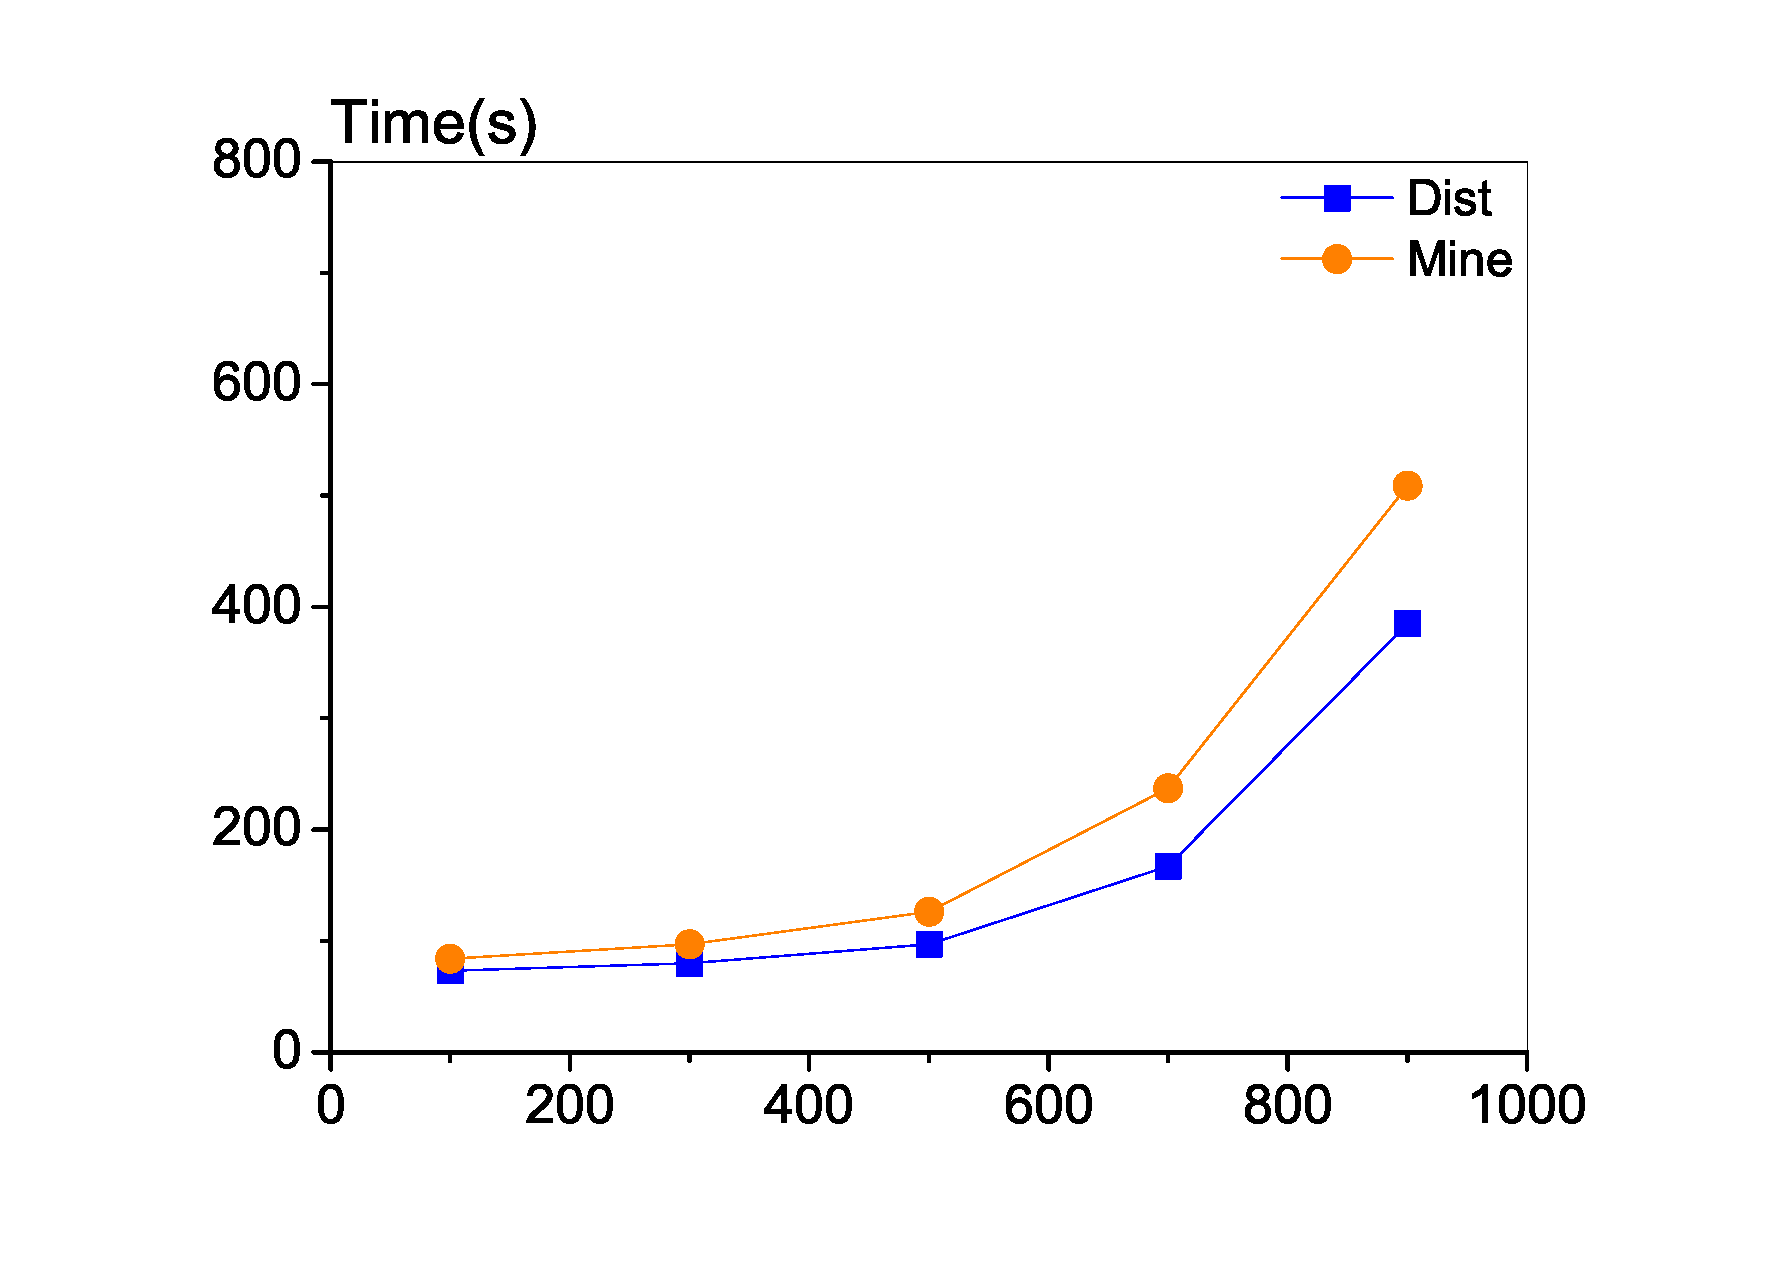
\includegraphics[width=7cm]{timebond.eps}
\end{minipage}%
}
\caption{Variation of $t_{max}$ ($\rho = 0.7$)}\label{fig:timebound}
\end{figure}

We choose $Retail$ as the target dataset again since $Retail$
is the most time-consuming dataset that can terminate within
acceptable time without DnC strategy.
The value of $t_{max}$ determines the size of a partition in DnC.
%Smaller $t_{max}$ can give rise to more partitions.
Here, we evaluate how partitioning helps with time performance and
its possible effects on suppression quality.
Figure \ref{fig:timebound-a} shows the relationship between partitions
and information loss. The lines of  $Dist$ is flat, indicating that
increasing $t_{max}$ doesn't cost us the quality of the solution. $Mine$
shows a slight descending tendency at first and then tends to be flat.
We argue that a reasonable $t_{max}$ will not cause our result quality to
deteriorate.
On the other hand, Figure \ref{fig:timebound-b} shows that
time cost increases dramatically  with the increase of  $t_{max}$.
The reason is that partitioning decreases the cost of enumerating \qids which
is the most time-consuming part in our algorithm. Moreover, parallel
processing is also a major reason for the acceleration.

\subsubsection{Variation of $b_{max}$}

\begin{figure}[tb]
\centering
\subfigure[Information Loss]{
\hspace{-1cm}
\begin{minipage}[c]{0.45\textwidth}
\centering
  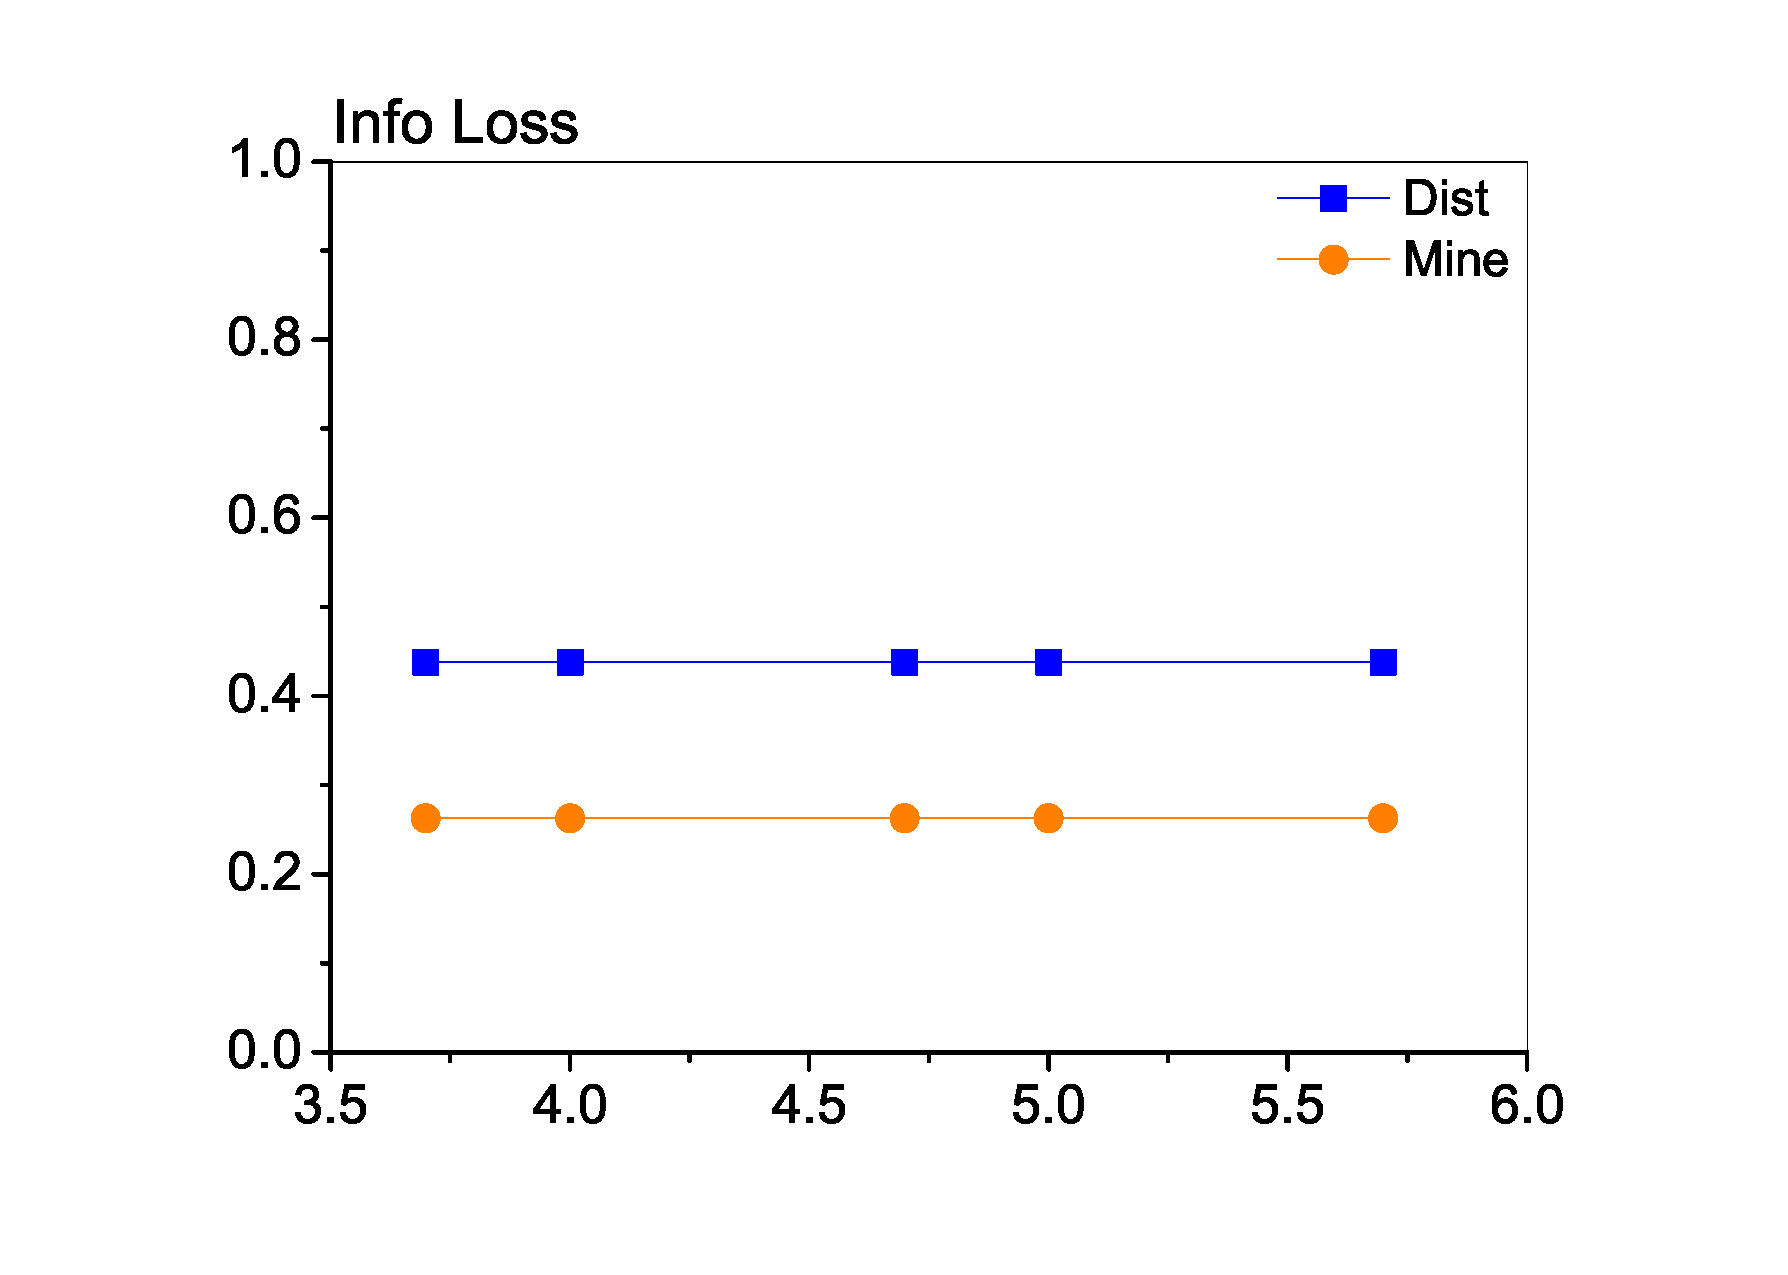
\includegraphics[width=7cm]{buffersizeavg.eps}
\end{minipage}%
}
\subfigure[Time Performance]{
\begin{minipage}[c]{0.45\textwidth}
\centering
  \includegraphics[width=7cm]{buffersize.eps}
\end{minipage}%
}
\caption{Variation of Buffer Size $b_{max}$ ($\rho=0.7$)}\label{fig:buffersize}
\end{figure}

Next experiment (See Figure \ref{fig:buffersize}) illustrates
the impact of varying $b_{max}$ on performance.
We choose $WV$ as our target dataset this time since the number of
distinct \qids in $WV$ is relatively small compared to
other datasets and our algorithm
can terminate even when we set a small $b_{max}$.

Note first that varying $b_{max}$ has no effect on
the information loss which
indicates that this parameter is purely for performance tuning.
At lower values, increasing $b_{max}$ gives almost exponential
savings in running time. But as $b_{max}$ reaches a certain point, the speedup
saturates, which suggests that given the fixed size of the data,
when $B$ is large enough to accommodate all \qids at once after some iterations,
further increase in $b_{max}$ is not useful.
The line for $Mine$ hasn't saturdated because $Mine$ suppresses
fewer items and retains more \qids, hence requires a much larger
buffer.

\subsection{A Comparison to Permutation Method}
In this section, we compare our algorithms with a permutation method
\cite{2011:TKDE:Anonymous}
which we call $M$.
The privacy model of $M$
states that the probability of associating any transaction $R \in T$ with
any sensitive item $e \in D_S(T)$ is below $1/p$, where $p$ is known as
a privacy degree. This model is similar to ours when $\rho = 1/p$,
which allows us to compare three variants of our algorithm against
$M$ where $p=4, 6, 8, 10$ on dataset $WV$ which was reported in
\cite{2011:TKDE:Anonymous}.
Figure \ref{fig:permutation1} shows the result on K-L divergence.
All variants of our algorithm outperform $M$ in
preserving the data distribution.
Figure \ref{fig:permutation2} shows timing results.
Even though $M$ is faster, our algorithms
terminate within acceptable time.

\begin{figure}[tb]
\centering
\subfigure[K-L Divergence]{\label{fig:permutation1}
\hspace{-1cm}
\begin{minipage}[c]{0.45\columnwidth}
%\flushleft
  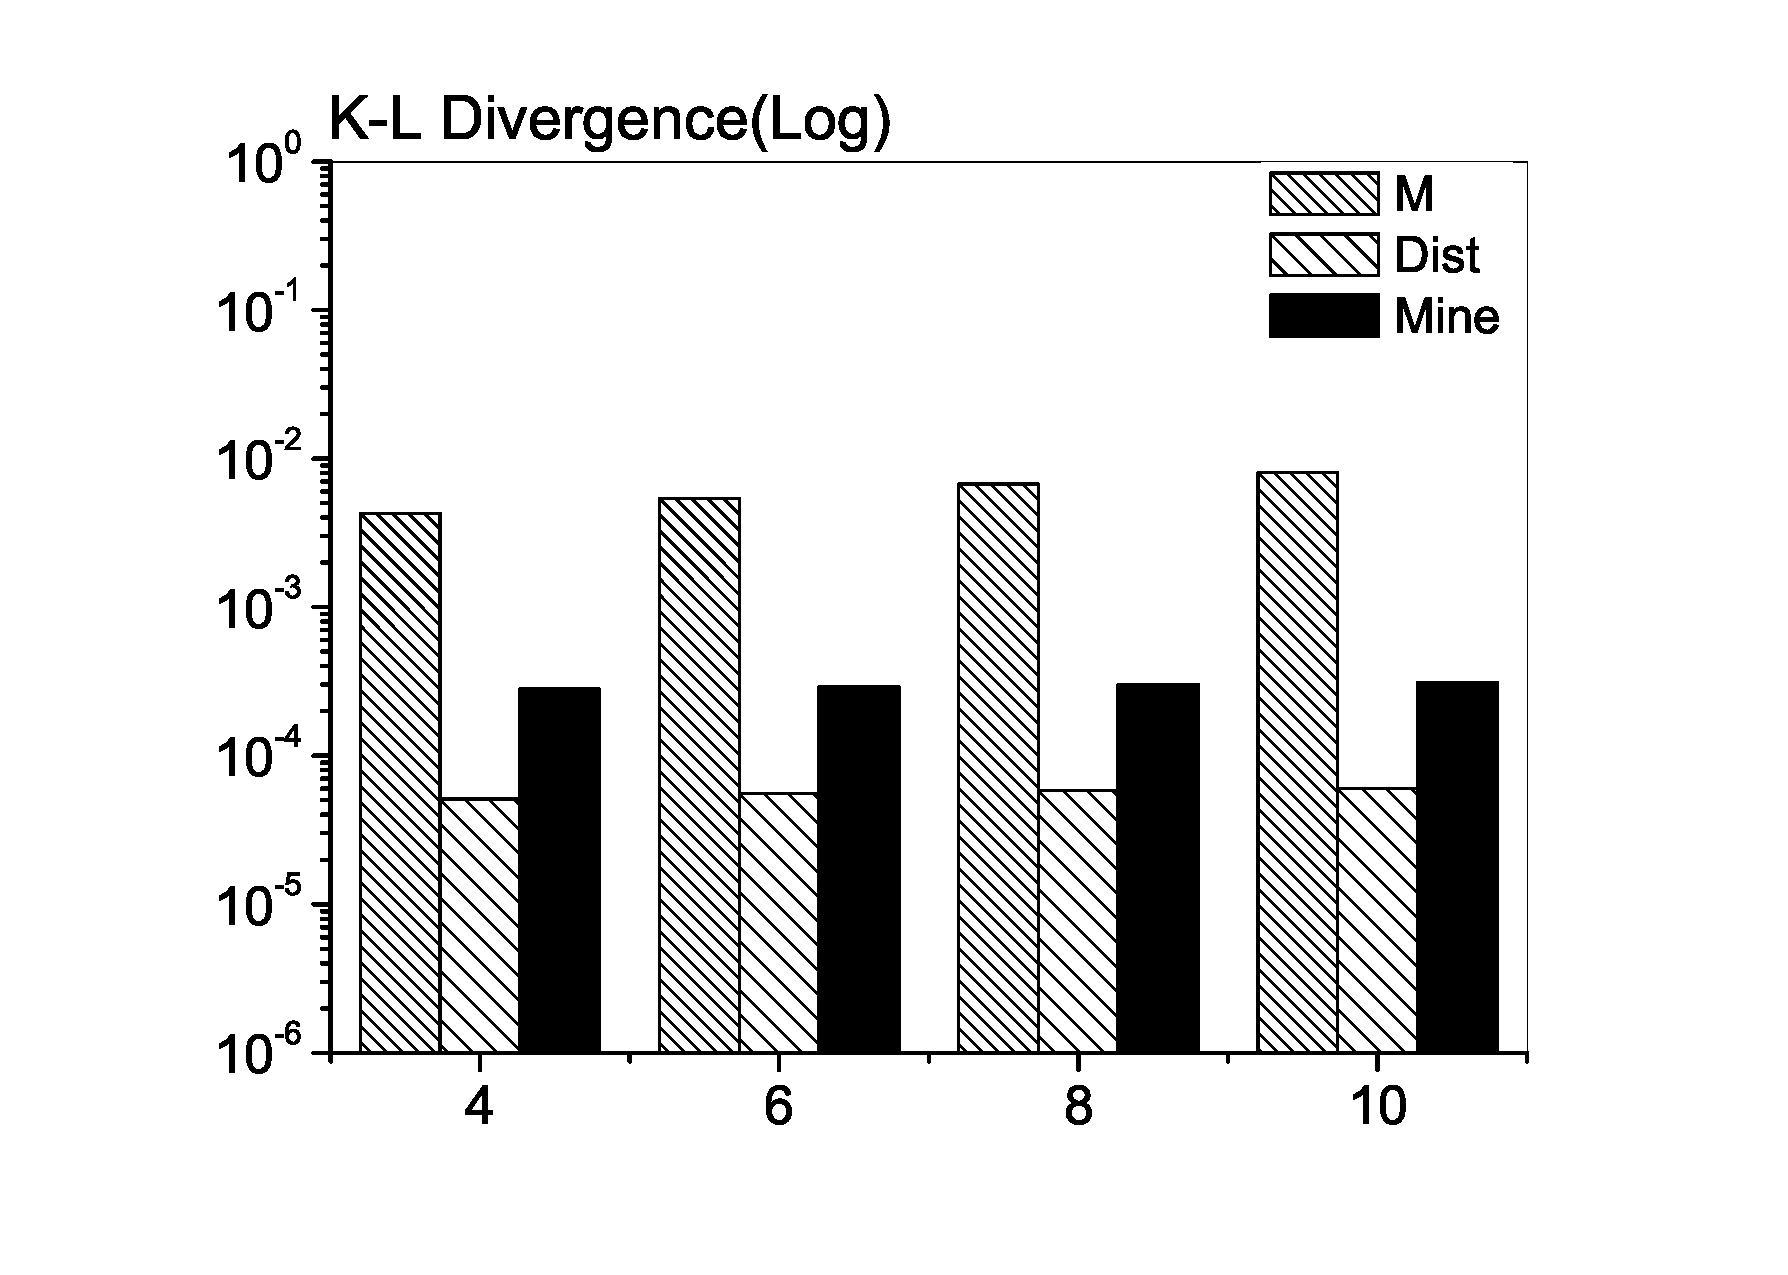
\includegraphics[width=7cm]{anatomy.eps}
\end{minipage}%
}
\subfigure[Time Performance]{\label{fig:permutation2}
\begin{minipage}[c]{0.45\columnwidth}
%\flushleft
  \includegraphics[width=7cm]{anatomytime.eps}
\end{minipage}%
}
\caption{Comparison with Permutation}
\end{figure}
